\documentclass[12pt]{article}

\usepackage[utf8]{inputenc}
\usepackage[russian]{babel}
\usepackage{amsmath, amssymb}
\usepackage{graphicx}
\usepackage{listings}

\lstset{
	language=Python,
	keepspaces=true,
	extendedchars=\true,
	inputencoding=utf8,
	basicstyle=\tiny,
	numbers=left,
	showspaces=false,
	showstringspaces=false,
}

\def\dd#1#2{\cfrac{\partial#1}{\partial#2}}

\author{Будакян Я. С.}

\begin{document}
	\begin{titlepage}
		\begin{center}
			{\small\textsc{Московский Государственный Университет им. М.\,В. Ломоносова}}
			\vskip 1pt \hrule \vskip 3pt
			{\small\textsc{Физический факультет}}
			\vfill
			{\Large Практическое задание по ОММ}
			\break
			\break
			{\Large Задача \#1}	
		\end{center}
		\vfill
		\begin{flushright}
			{Выполнил студент 335 группы\\Будакян Я.\,С.\\
			 Преподаватель Домбровская Ж.\,О.}
		\end{flushright}
	\end{titlepage}
	
	\section{Постановка задачи}
		\bigskip\par\noindent{\bf Задача 2. }
		Используя схему бегущего счета и итерационные методы, решить задачу:
		\begin{equation}\label{eq:problem}
			\begin{cases}
				&\dd{u}t - u\dd{u}x = 0, \quad -1 \le x < 0, \\
				&u(x, 0) = 2 - \frac{4}{\pi}\arctg(x+2), \\
				&u(0, t) = (2 - \frac{4}{\pi}\arctg2)e^{-t}
			\end{cases}
		\end{equation}
	
	\section{Метод решения}
		Во первых, чтобы определить, нет ли у решения разрыва, необходимо составить уравнение характеристик и посмотреть, пересекаются ли они:
		$$ \frac{dt}{1} = \frac{dx}{-u} = \frac{du}{0},$$
		откуда получаем:
		$$ du = 0 \rightarrow u = const,$$
		$$ dt = -\frac{1}{u}dx \rightarrow t - t_0 = -\frac{1}{u}(x - x_0)$$
		Подставив начальные условия, получаем уравнения для характеристик, выходящих из оси t:
		\begin{equation}\label{char_t0}
			x = (\frac{4}{\pi}\arctan2-2)(t-t_0)e^{-t_0},
		\end{equation}
		и оси x:
		\begin{equation}\label{char_x0}
			x = x_0 - t(2 - \frac{4}{\pi}\arctan(x_0+2))
		\end{equation}
		Построим графики семейств характеристик:
		\newpage
		\begin{figure}[h]
			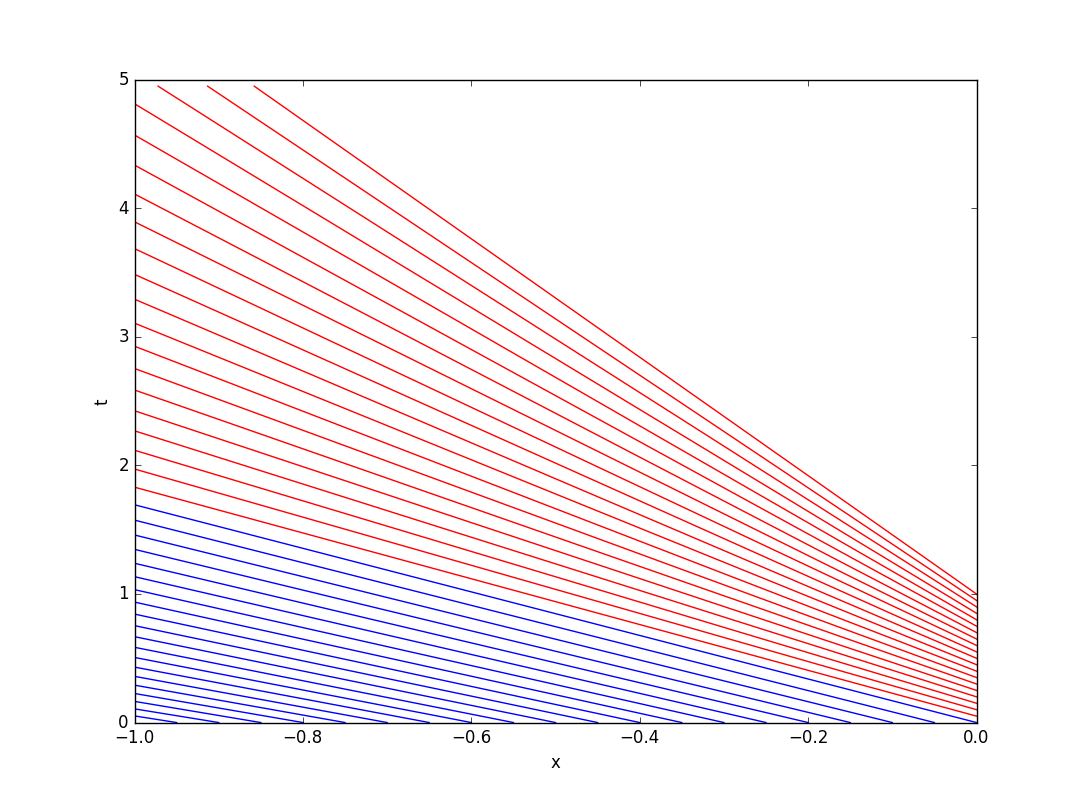
\includegraphics[scale = 0.5]{char_1}
			\caption{Семейства характеристик, красные соответствуют (\ref{char_t0}), синие - (\ref{char_x0})}
		\end{figure}
		Как видно из рисунка, в рассматриваемой области $ -1 \leq x < 0 $ характеристики не пересекаются. Следовательно, временной интервал расчета может быть выбран произвольно, например, $t \in [0, 1]$.
		Введем равномерные разностные сетки:
		$$\bar{\omega}_h = \{x_i = ih;\ i = \overline{0,N};\ hN = 1\}$$
		$$\bar{\omega}_\tau = \{t_j = j\tau;\ j =\overline{0,S};\ \tau S = T\}$$
		$$\bar{\omega}_{h\tau} = \bar{\omega}_h \times \bar{\omega}_\tau = 
		\{ (x_i, t_j) \in \bar{D} \}$$
		$$\bar{D} = \{ -1 \le x < 0;\ 0 \le t \le T \}$$
		
		Перепишем основное уравнение (\ref{eq:problem}) в дивергентном виде:
		$$\dd{u}t + \dd{}x\left(\frac{-u^2}{2}\right) = 0$$
		Введем сеточную функцию:
		$$y_{ij} \overset{\mathrm{def}}{=} u(x_i, t_j)$$
		Запишем разностную схему задачи (\ref{eq:problem}), используя неявный четырехточечный шаблон с весовыми пространственными и временными производными с весом $\sigma = \frac{1}{2}$ :
		\begin{figure}[h!]
			\begin{center}
				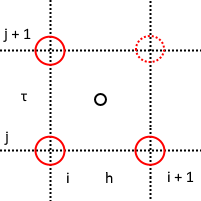
\includegraphics[width=0.5\linewidth]{template}
				\caption{Шаблон "прямоугольник"\,, i - x, j - t}
			\end{center}
		\end{figure}
		$$\dd{u}t \to $$
		

\end{document}
